\section{Tutorial 3 (Sept 26, 2025)}

\begin{problem}

\end{problem}

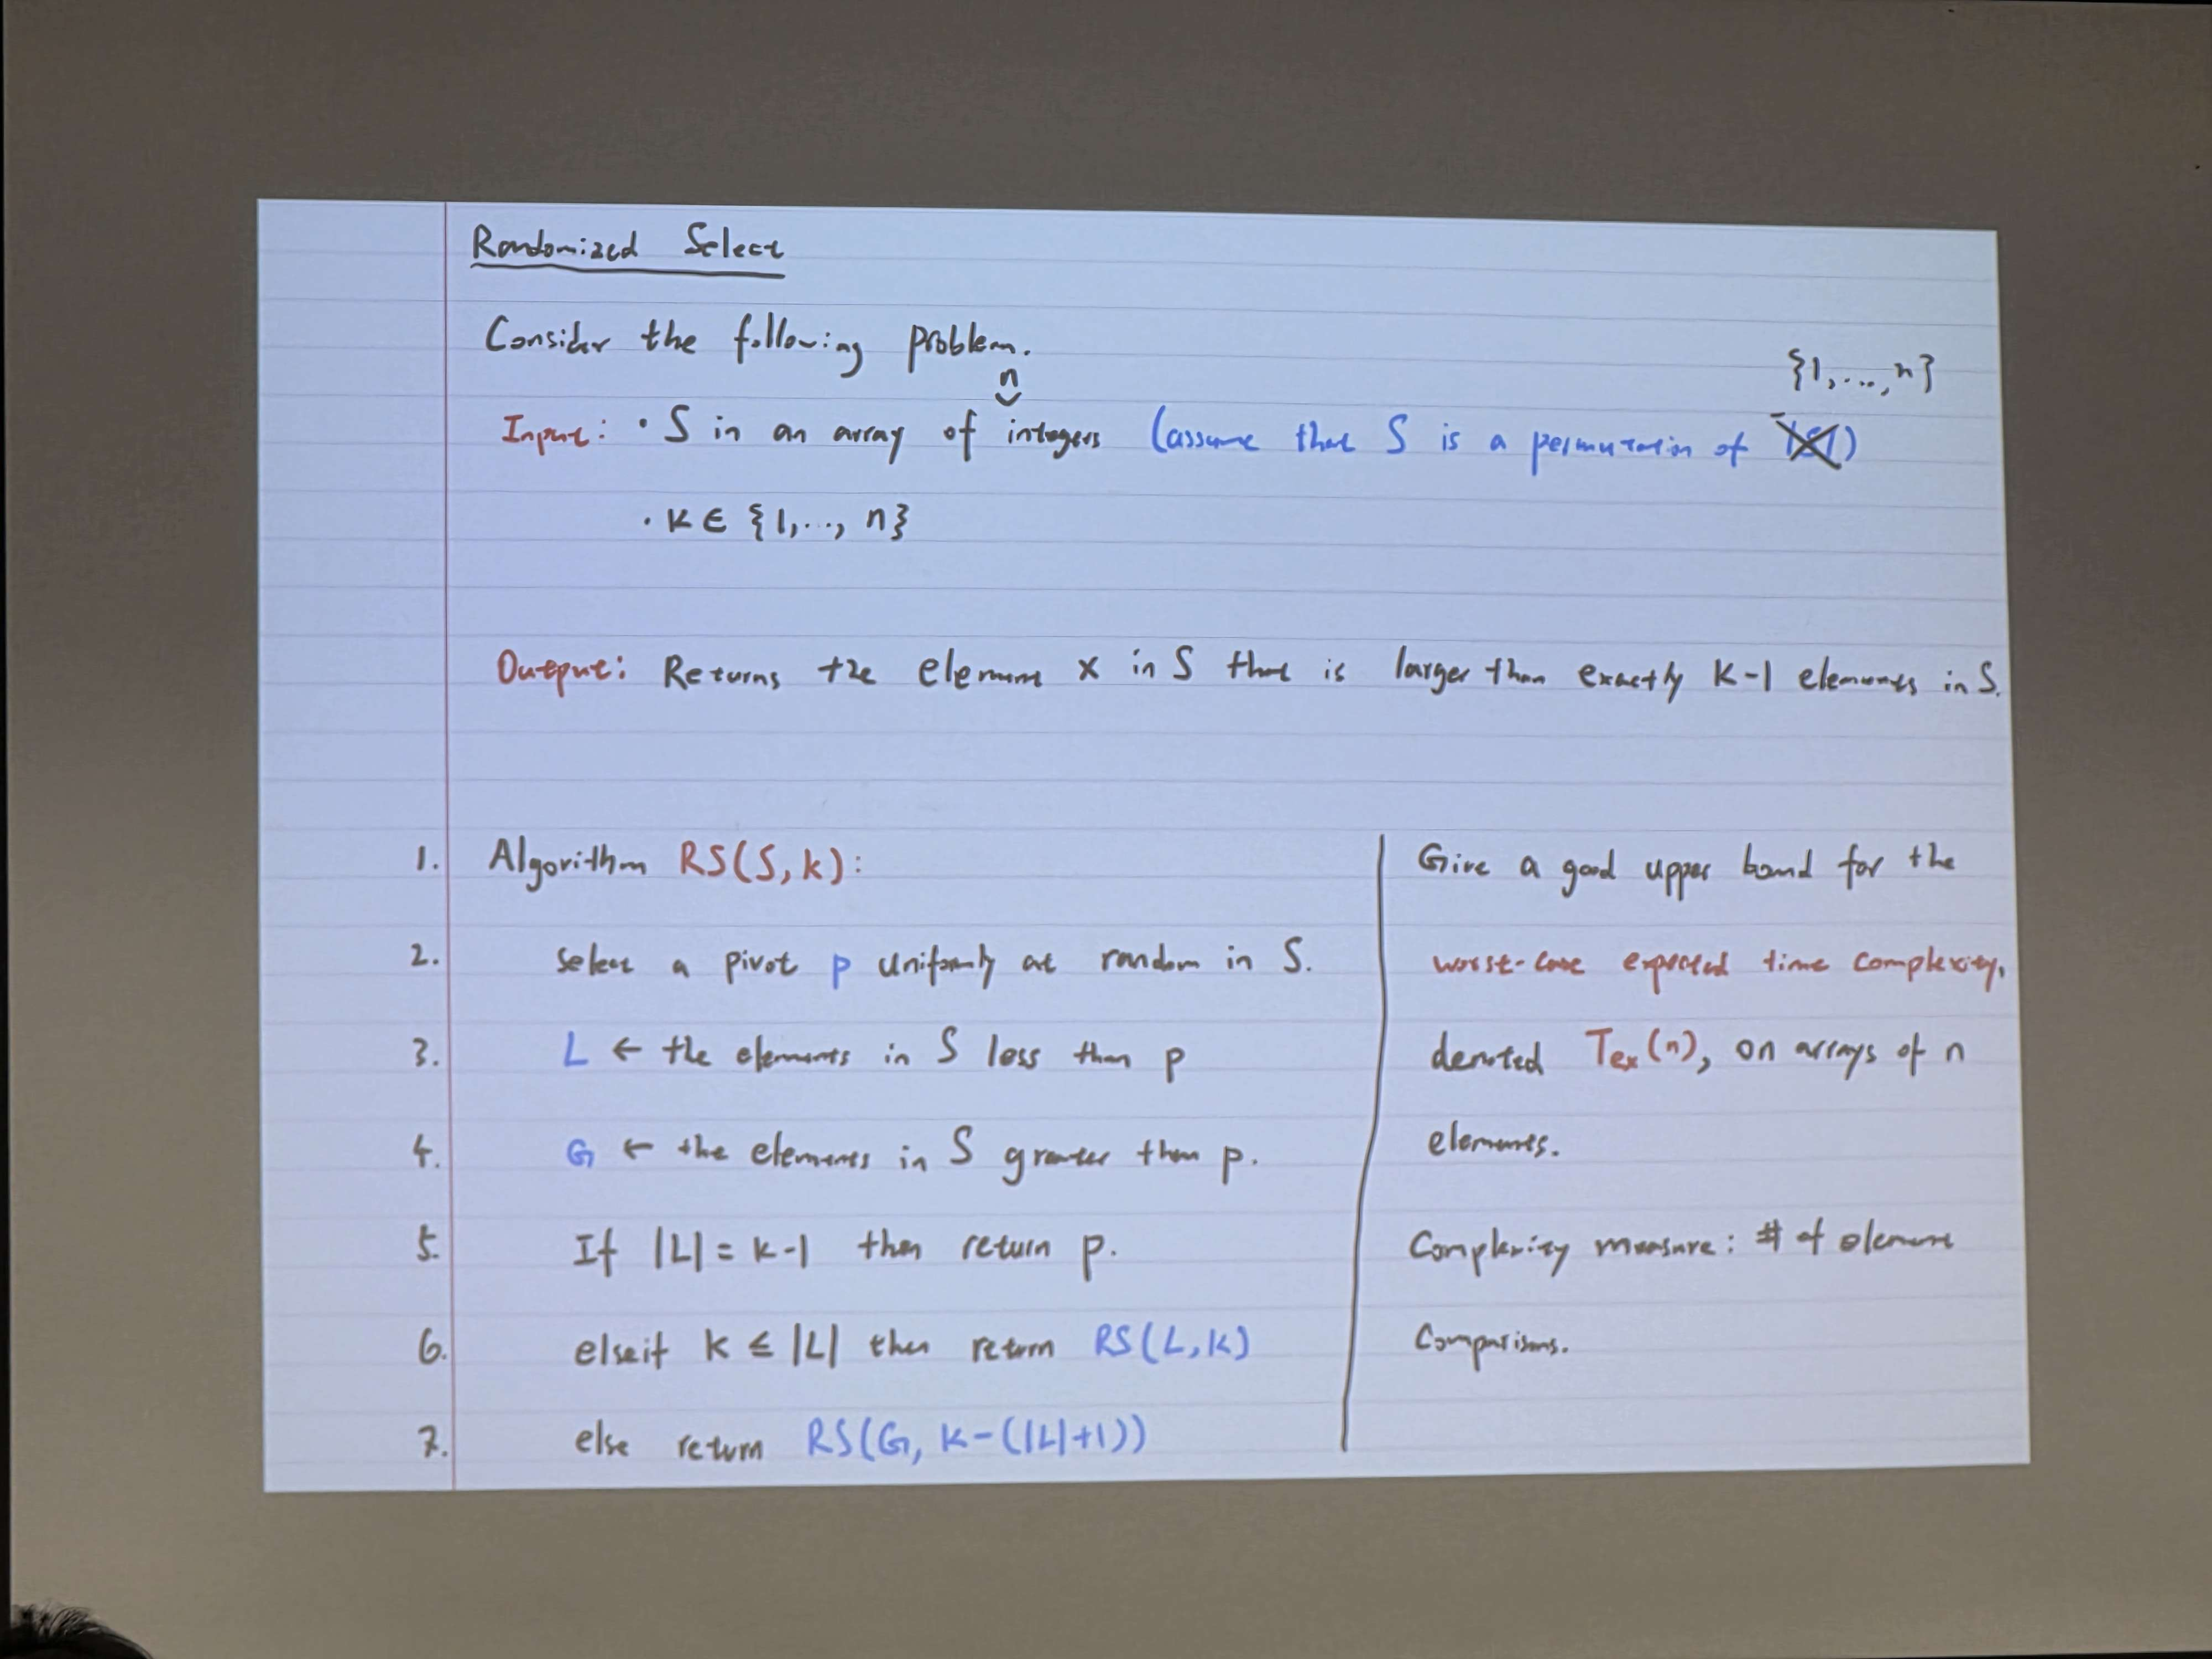
\includegraphics{csc265/figures/tut3.jpg}

We want to count the number of comparisons. We must first define a random variable, let us define $X_{i, j, k}(\alpha)$ be the indicator variable for if a comparison between element $i$ and $j$ occurred when $\alpha$ is the sequence of random pivots chosen by the algorithm, with $k$ being the pivot picked. Then
\[
t_n(\alpha) = \sum_{1 \leq i < j \leq n} X_{i, j, k}(\alpha)
\]
thus
\[
T_{EX}(n) = \underset{\alpha}{\mathbb{E}}[t_n(\alpha)] = \sum_{1 \leq i < j \leq n} \underset{\alpha}{\mathbb{E}}[t_n(\alpha)] = \sum_{1 \leq i < j \leq n} \text{Pr}[X_{i, j, k} = 1]
\]
We partition into cases as follows:

\noindent \textit{Case $i < j < k$}:
We realize that any contiguous part of $\{ i, \cdots, k \}$ `remains together' through successive recursive calls, until the first time a pivot is chosen among them.

Let $p$ be the new pivot that is chosen. If $p \ne i$ and $p \ne j$, then $i$ and $j$ are not compared, since $j$ would be in $G$, and $i$ would be in $L$. However, if $p = i$ or $p = j$, then $p$ is compared against the rest of $S$, so the comparison between $i$ and $j$ must occur. 
\[
\text{Pr}[X_{i, j, k} = 1] = \text{Pr}[p = i \text{ or } p = j] = 2 \cdot \frac{1}{k - i + 1}
\]

\noindent \textit{Case $k < i < j$}

This case is similar, giving us $\text{Pr}[X_{i, j, k} = 1] = 2 \cdot \frac{1}{k - i + 1}$
